% !TeX spellcheck = it_IT
\documentclass[12pt, answers]{exam}

\usepackage[hidelinks]{hyperref}
\usepackage{xcolor}
\definecolor{bg}{rgb}{0.95,0.95,0.95}
\definecolor{g}{rgb}{0,0.5,0.1}
\usepackage{minted}
\setminted[c]{bgcolor=bg}
\setminted[python]{linenos, bgcolor=bg}
\setminted[java]{bgcolor=bg}
\usepackage[autostyle, english = american]{csquotes}
\MakeOuterQuote{"}
\usepackage{array}
\usepackage{tcolorbox}
\usepackage{algorithm2e}
\usepackage{amsmath}
\usepackage{amsfonts}

\title{GPU Computing}
\author{Massimo Perego}
\date{}

\renewcommand{\contentsname}{Sezioni}
\newcommand{\N}{\mathbb{N}}
\newcommand{\tc}{\, \text{ t.c. } \,}

% TODO: Domande trovate (fuori da Notion)

% Pattern
%- NSY: mostrare il pseudo codice dell'algoritmo di boruvka
%- NSY: Fare uno schema di una BFS parallela

% Domande in dubbio:
% - schema di utilizzo di più gpu, ad esempio per la somma di due vettori
%		Lo ha spiegato?
% - Sincronizzazione a due livelli di CUDA.
% 		Cosa vuol dire?
% - Uso degli stream per il prodotto di matrici diagonali a blocchi.
%		Non penso lo abbia spiegato? Ho un fever dream a riguardo, ma non trovo nulla al momento

\begin{document}
    
\maketitle

\tableofcontents

\newpage
    
% !TeX spellcheck = it_IT
\section{Sincronizzazione}

\begin{questions}
    \question Quali sono i meccanismi di sincronizzazione?
    
    \begin{solution}
        Si possono avere più \textbf{livelli di sincronizzazione}:
        \begin{itemize}
            \item \textbf{Livello di sistema}: per attendere che un dato task venga completato su host e device; la primitiva
            \begin{minted}{c}
cudaError_t cudaDeviceSynchronize(void);
            \end{minted}
            blocca l'applicazione host finché tutte le operazioni CUDA su tutti gli stream non sono completate. Si tratta di una funzione host-side only (una volta usata lato device per gestire il parallelismo dinamico, ma ora deprecata);
            
            \item Non c'è una primitiva esplicita per la sincronizzazione a \textbf{livello di grid}, ma la si può ottenere (da CC 6 in avanti) lanciando un kernel cooperativo
            \begin{minted}{c}
cudaLaunchCooperativeKernel(
    (void*)myKernel,
    gridDim, blockDim,
    kernelArgs, /*sharedMemBytes=*/0, /*stream=*/0);
            \end{minted}
            e all'interno del kernel
            \begin{minted}{c}
grid_group grid = this_grid();
// work work work ...
// waits for _all_ blocks in *this* kernel
grid.sync();
            \end{minted}
            Non ci devono essere ulteriori kernel attivi all'interno del device;
            
            \item \textbf{Livello di blocco}: per attendere che tutti i thread in un blocco raggiungano lo stesso punto di esecuzione. La primitiva
            \begin{minted}{c}
__device__ void __syncthreads(void);
            \end{minted}
            impone a tutti i thread nel blocco corrente di attendere fino a quando tutti gli altri thread dello stesso blocco non hanno raggiunto quel particolare punto di esecuzione. Lo scopo principale è garantire la visibilità degli accessi alla memoria (rendere visibile le modifiche), in modo da evitare conflitti e race conditions. Se non tutti i thread all'interno del blocco arrivano alla primitiva si può avere un deadlock;
            
            \item \textbf{Livello di warp}: per attendere che tutti i thread all'interno di un warp raggiungano lo stesso punto di esecuzione. La primitiva
            \begin{minted}{c}
__device__ void __syncwarp(mask);
            \end{minted}
            permette di avere una barriera esplicita per garantire la ri-convergenza del warp per le istruzioni successive. L'argomento \texttt{mask} è composto da una sequenza di 32 bit che permette di definire quali warp partecipano alla sincronizzazione (se omessa, di default tutti, ovvero \texttt{0xFFFFFFFF}).
        \end{itemize}
        
        Sincronizzazione \textbf{tramite stream}: tra stream non-NULL diversi non si ha nessuna dipendenza od ordinamento, mentre lo stream di default (\texttt{0}) ha un comportamento diverso, può essere: 
        \begin{itemize}
            \item legacy: bloccante rispetto a tutti gli altri stream, un'operazione lanciata nel default stream non può iniziare finché non sono completate tutte le operazioni precedenti in qualsiasi altro stream (e viceversa);
            
            \item per-thread: disponibile da CUDA 7, ogni thread host ottiene il suo default stream, diventa non-bloccante rispetto agli altri stream
        \end{itemize}
        
        Sincronizzazione \textbf{tramite eventi}: all'interno degli stream si possono creare degli eventi tramite i quali è possibile avere anche sincronizzazione:
        \begin{itemize}
            \item Host-side: la primitiva
            \begin{minted}{c}
cudaError_t cudaEventSynchronize(cudaEvent_t event);
            \end{minted}
            permette di attendere lato host finché l'evento specificato non viene completato; esiste una variante non-bloccante:
            \begin{minted}{c}
cudaError_t cudaEventQuery(cudaEvent_t event)
            \end{minted}
            che permette di controllare se un evento è stato completato o meno, senza bloccare l'host;
            
            \item Stream-to-stream: per far attendere a uno stream il completamente di un evento su un altro stream. La primitiva:
            \begin{minted}{c}
cudaError_t cudaStreamWaitEvent(
    cudaStream_t stream , cudaEvent_t event);
            \end{minted}
            permette di aspettare un evento su un altro stream (anche su altri device).
        \end{itemize}
        
        Sincronizzazione \textbf{implicita} dovuta a operazioni bloccanti: alcune operazioni causano sincronizzazione in quanto implicano un blocco su tutte le operazioni precedenti sul device corrente. In questo gruppo rientrano molte operazioni relative alla gestione della memoria.
        
        %Ignorerà le primitive di sincronizzazione dei cooperative groups, non spiegate?
    \end{solution}
    
    \question Meccanismi di sincronizzazione tra GPU e modalità di trasmissione tra queste.
    
    \begin{solution}
        Tra diverse GPU ci sono più metodi di \textbf{sincronizzazione} possibili: 
        \begin{itemize}
            \item Il metodo più semplice è lasciare che sia l'host a sincronizzare tutte le GPU, la primitiva \texttt{cudaDeviceSynchronize()} permette di attendere il completamento di tutte le operazioni su tutte le GPU (il comando va ripetuto per ogni device)
            
            \item Per una gestione più flessibile si possono usare gli eventi CUDA; un evento è un marcatore all'interno di una stream su un device, un'altra GPU può "ascoltare" per attendere il completamento di un evento su un altro device, tramite \texttt{cudaStreamWaitEvent()} (bloccante) o \texttt{cudaStreamQueryEvent()} (non bloccante)
            
            \item La libreria NCCL (Nvidia Collective Communications Library) fornisce primitive di comunicazione con sincronizzazione implicita
        \end{itemize}
        
        Anche per \textbf{trasmettere dati} tra più GPU ci sono diverse modalità:
        \begin{itemize}
            \item La più semplice è via host: i dati vengono copiati sull'host e poi passati ai device a cui servono (tramite \texttt{cudaMemcpy()})
            
            \item Se il P2P è abilitato, esistono primitive che permettono lo scambio dati tra GPU diverse, come ad esempio \texttt{cudaMemcpyPeer()}; esistono anche primitive asincrone come \texttt{cudaMemcpyAsync()} e \texttt{cudaMemcpyPeerAsync()}
            
            \item Usare unified memory: la memoria unificata permette di avere uno spazio di indirizzamento condiviso tra host e device, allocando con \texttt{cudaMallocManaged()} si può usare lo stesso puntatore su tutti i dispositivi
            
            \item Per primitive di comunicazione altamente ottimizzate per la comunicazione collettiva la libreria NCCL offre throughput elevato e bassa latenza
        \end{itemize}
    \end{solution}
\end{questions}

% !TeX spellcheck = it_IT
\section{Memoria}

\begin{questions}
    \question Cosa sono local e constant memory?
    
    \begin{solution}
        In CUDA è presente una gerarchia di memorie, con diversi tipi di memoria al suo interno, ciascuno con dimensioni, banda e scopi specifici. 
        
        Local e constant memory sono due tipi di memoria programmabile esposti al programmatore: 
        \begin{itemize}
            \item \textbf{Local memory}: memoria off-chip (quindi molto lenta), locale ai thread; risiede in global memory. Da CC 2.0 parti di questa sono in cache L1 e L2.
            
            Viene usata per variabili "grandi" (o la cui dimensione non è nota a compile time), oltre che per lo spilling dei registri (quando il kernel usa troppe variabili).
            
            \item \textbf{Constant memory}: si tratta di uno spazio di memoria di sola lettura, accessibile da tutti i thread. La si può dichiarare usando il qualificatore \texttt{\_\_constant\_\_}. Sono 64k per tutte le CC off-chip, con 8k di cache dedicata in ogni SM. Ha scope globale va dichiarata staticamente al di fuori dei kernel.
            
            Viene usata quando tutti i thread devono leggere dalla stessa locazione (raggiunge l'efficienza dei registri); in altri casi le performance sono significativamente minori.
        \end{itemize}
        
        In sintesi: local memory è lenta, serve quando registri e shared memory non bastano, la constant memory è una zona di sola lettura, ideale per accessi broadcast a piccole tabelle condivise.
    \end{solution}
    
    \question Cosa sono le memorie pinned, zero copy e unified.
    
    \begin{solution}
        La memoria \textbf{pinned} è memoria host non paginabile dal sistema operativo, ovvero non può essere fatto lo swap su disco di quella zona di memoria. La si può allocare con \texttt{cudaHostAlloc()}, permette trasferimenti asincroni con maggiore throughput rispetto alla memoria paginabile (evita overhead dovuto al pinning temporaneo). Da notare che l'allocazione eccessiva potrebbe degradare le performance host.
        
        La memoria \textbf{zero copy} si basa su memoria pinned mappata nello spazio di indirizzamento del device, permette alla GPU di accedere direttamente a pagine di memoria host senza copie esplicite di memoria. Può semplificare la programmazione, ma ha latenza più alta della global memory (i dati devono passare su PCIe) e banda limitata.
        
        La memoria \textbf{unified} è un modello di memoria automatico in cui host e device condividono lo spazio di indirizzamento, tutte le CPU e GPU del sistema possono accedere a questa memoria. Il sistema sottostante si occupa di gestire le migrazioni di memoria secondo necessità, in maniera trasparente all'applicazione. Può essere allocata con \texttt{cudaMallocManaged()} e permette di semplificare notevolmente la programmazione, evitando tutte le copie di dati esplicite, ma si ha overhead di migrazione quando viene fatto l'accesso ai dati.
    \end{solution}
    
    \question Modalità di accesso alla device memory e performance.
    
    \begin{solution}
        In CUDA si ha una gerarchia di memorie: 
        \begin{itemize}
            \item Registri: allocati per thread, estremamente veloci (latenza praticamente nulla), ma hanno capienza limitata e un uso eccessivo porta a spilling in memoria locale
            
            \item Shared Memory: memoria condivisa tra i thread di uno SM, latenza bassa, organizzata in bank: accessi senza conflitti di bank garantiscono throughput massimo. Dimensione comunque limitata e l'uso che ne fa ogni blocco determina il numero di blocchi che possono essere in esecuzione su uno SM concorrentemente
            
            \item Global Memory: memoria più grande e a più alta latenza ($400 \sim 800$ cicli), accessibile da tutti i thread e dall'host. Permette un buon throughput, ma solo se gli accessi sono coalescenti (raggruppati in transazioni larghe)
            
            \item Local Memory: risiede fisicamente nella global memory, quindi ha la stessa latenza, viene usata per variabili molto grandi o per lo spilling dei registri
            
            \item Constant \& Texture memory: risiedono nella device memory, ma hanno una cache all'interno di ogni SM, sono usate per accessi uniformi read-only, ovvero quando tutti i thread devono accedere a una stessa zona di memoria (hanno la banda della device memory altrimenti). La texture memory è ottimizzata per dati e operazioni su dati espressi sotto forma di matrici
        \end{itemize}
    \end{solution}
    
    \question Memorie statiche e dinamiche.
    
    \begin{solution}
        Le allocazioni di memoria possono essere statiche o dinamiche. Le allocazioni statiche hanno dimensione nota compile-time e possono risiedere a livello di: 
        \begin{itemize}
            \item Global memory: la si può dichiarare tramite \texttt{\_\_device\_\_} (o \texttt{\_\_constant\_\_} se di sola lettura), ha un accesso lento, scope e lifetime globale
            
            \item Shared memory: la si può dichiarare tramite \texttt{\_\_shared\_\_} all'interno del kernel, latenza bassa, ha scope a livello di blocco e lifetime del kernel
            
            \item Registri: variabili locali ai thread, si tratta della memoria più veloce, ma di dimensione limitata
        \end{itemize}
        
        Le allocazioni dinamiche invece sono usate quando la dimensione dei dati è nota solo in esecuzione. Possono essere:
        \begin{itemize}
            \item Device malloc: tramite la primitiva \texttt{cudaMalloc()}, richiede passaggi di memoria espliciti da host a device (e viceversa, \texttt{cudaMemcpy()}), disponibile fino all'istruzione \texttt{cudaFree()}, risiede nella memoria globale del device
            
            \item Pinned memory: non all'interno del device, ma la primitiva \texttt{cudaHostAlloc()} permette di allocare memoria non paginabile dal sistema operativo per trasferimenti più veloci; questa può essere mappata nello spazio di indirizzamento della GPU (memoria zero copy)
            
            \item Unified Memory: la primitiva \texttt{cudaMallocManaged()} permette di avere una zona di memoria con indirizzamento unico per host e device, lasciando la gestione della migrazione dei dati a CUDA; semplice da utilizzare, ma può portare a maggiori latenze se non usata correttamente
            
            \item Shared memory: la memoria condivisa può essere allocata dinamicamente tramite una dichiarazione all'interno del kernel di una variabile adimensionale:
            \begin{minted}{cuda}
extern __shared__ float s[];
            \end{minted}
            Va poi passato come terzo argomento tra variabili angolari durante il lancio del kernel la dimensione della memoria condivisa:
            \begin{minted}{cuda}
kernel<<<grid, block, shared_bytes>>>();
            \end{minted}
        \end{itemize}
    \end{solution}
    
    \question Significato e uso della memoria unificata.
    
    \begin{solution}
        La memoria unificata è un modello di gestione della memoria che permette l'utilizzo di un singolo spazio di indirizzamento (puntatore unico) per accedere a dati sia host che device. 
        
        Ha lo scopo di semplificare la gestione della memoria, rendendo trasparenti al programmatore i trasferimenti, gestiti da CUDA. 
        
        La si può allocare tramite la funzione \texttt{cudaMallocManaged()}, è anche presente un parametro \texttt{flag} per specificare se la memoria è condivisa solo con l'host o anche con tutte le altre GPU.
        
        Semplifica lo sviluppo CUDA, ma può portare a un maggiore overhead dovuto alla migrazione (gestita a livello di pagina) rispetto alla gestione della memoria con trasferimenti espliciti.
    \end{solution}
    
    \question Significato e utilità di pattern di accesso alla memoria globale. Distinzioni tra lettura e scrittura.
    
    \begin{solution}
        La global memory è una memoria off-chip (DRAM, divisa dal chip dell'SM su cui il thread è in esecuzione), quindi ad alta latenza ($400\sim 800$ cicli di clock), con scope e lifetime globale. 
        
        I pattern di accesso alla memoria globale sono le strutture riguardanti "come" viene effettuato l'accesso alla memoria da parte dei thread. La global memory ha, infatti, latenza elevata, ma throughput ampio quando gli accessi sono coalescenti.
        
        Gli accessi alla memoria del device possono avvenire in transazioni da 32, 64 o 128 byte. Spesso le applicazioni sono limitate dal throughput effettivo della memoria, quindi per rendere efficienti i trasferimenti si vuole minimizzare il numero di transazioni. 
        
        Per migliorare le prestazioni è bene ricordare che le istruzioni vengono eseguite a livello di warp, per un dato indirizzo si esegue una operazione di loading/storing e i 32 thread presentano una singola richiesta di accesso, da servire in una o più transazioni.
        
        Gli accessi possono essere:
        \begin{itemize}
            \item Allineati: quando il primo indirizzo della transazione è un multiplo della granularità della memoria usata per servire la transazione (32 byte per L1, 128 per L2)
            
            \item Coalescenti: quando i 32 thread accedono a un blocco contiguo di memoria
        \end{itemize}
        
        Per sfruttare al meglio le transazioni di memoria bisogna rispettare allineamento e coalescenza. Al contrario, effettuare accessi non coalescenti/strided significa rendere necessarie più transazioni per la stessa quantità di dati (fino a 32 diverse).
        
        Può essere importante strutturare i dati in modo da avere accessi coalescenti (array of structures vs structures of array).
        
        Le operazioni di scrittura non usano la cache L1, le \texttt{store} vengono cachate solo in L2, prima di essere inviati alla device memory in 1, 2 o 4 segmenti da 32 byte. Accessi allineati e coalescenti sono ugualmente importanti per lettura e scrittura. Inoltre, per la sola lettura esistono zone di memoria dedicate (constant e texture memory); in generale la lettura possiede una gerarchia di memorie più complessa.
    \end{solution}
    
    \question Bank e bank conflict.
    
    \begin{solution}
        La shared memory è una memoria condivisa a livello di blocco, locata all'interno dello SM. Questa è organizzata in "banks" paralleli che permettono l'accesso simultaneo ai dati.
        
        La shared memory è quindi suddivisa in blocchi identici, solitamente da 4 byte/una word, e ciascun blocco può servire un solo accesso per ciclo di clock. 
        
        Se più thread accedono in parallelo a indirizzi mappati a bank diversi, questi accessi possono avvenire in parallelo, altrimenti, se due o più thread vogliono accedere allo stesso bank si ha un bank conflict e gli accessi vengono serializzati. Si vogliono quindi evitare i conflitti per utilizzare la massima banda disponibile.
    \end{solution}
    
    \question Constant memory e il suo utilizzo.
    
    \begin{solution}
        Si tratta di una memoria che risiede nella device memory, con una cache dedicata per ogni SM. La si può definire tramite l'attributo \texttt{\_\_constant\_\_}, permette di ospitare dati di sola lettura, ideale per accessi uniformi. Ha scope globale, va dichiarata al di fuori dei kernel e staticamente.
        
        Ideale per quando tutti i thread all'interno di un warp devono leggere dallo stesso indirizzo di memoria, raggiungendo efficienza simile a quella dei registri, altrimenti le letture vengono serializzate, degradando significativamente le performance.
        
        Può essere inizializzata dall'host usando
        \begin{minted}{cuda}
cudaError_t cudaMemcpyToSymbol(const void* symbol,
    const void* src, size_t count);
        \end{minted}
        Si può anche leggere lato host tramite
        \begin{minted}{cuda}
cudaError_t cudaMemcpyFromSymbol(const void* dst, 
    const void* symbol, size_t count);
        \end{minted}
    \end{solution}
    
    \question Come viene mappata logicamente e fisicamente la shared Memory.
    
    \begin{solution}
        La shared memory è una memoria programmabile a bassa latenza, con scope di blocco (visibile da tutti thread all'interno di uno stesso blocco) e lifetime pari a quello del kernel. La si può dichiarare tramite il qualificatore \texttt{\_\_shared\_\_}, sia staticamente che dinamicamente (aggiungendo \texttt{extern} e specificando la dimensione in fase di chiamata del kernel). Serve come comunicazione a bassa latenza tra thread dello stesso blocco. La dimensione della shared memory è limitata e il numero di blocchi concorrenti è determinato anche dalla smem disponibile.
        
        Fisicamente, si tratta di una memoria on-chip, quindi posizionato sullo stesso chip dello SM, organizzata linearmente in moduli chiamati bank (tipicamente 32). Gli accessi alla shared memory (sia \texttt{load} che \texttt{store}) vengono emessi per warp e la banda massima si ha quando tutti gli warp accedono a bank diversi (word consecutive). Se due thread all'interno dello stesso warp tentano di accedere allo stesso bank si ha un bank conflict, che richiede la serializzazione degli accessi e causa un degrado delle prestazioni.
    \end{solution}
    
    \question Vantaggi della Unified Memory ed esempio di utilizzo.
    
    \begin{solution}
        La memoria unificata (unified memory), introdotta da CUDA 6.0, semplifica la gestione della memoria creando uno spazio di indirizzamento unico tra CPU e GPU. Tramite un unico puntatore si può accedere sia alla memoria host che device. 
        
        Il trasferimento di dati avviene in maniera trasparente al programmatore, gestito dal sistema CUDA. Tra i vantaggi possiamo notare:
        \begin{itemize}
            \item semplicità di programmazione, si tratta di un modello più semplice, non richiede gestione manuale della memoria e porta a codice più comprensibile
            
            \item coerenza automatica della memoria, CUDA si occupa di mantenere automaticamente la coerenza tra host e device, a volte a scapito delle performance
            
            \item over-subscription della memoria, si può allocare più memoria di quanta sia fisicamente disponibile sulla GPU, le pagine verranno spostate in automatico quando necessario, permettendo di usare data set più grandi
        \end{itemize} 
        
        Esempio di utilizzo:
        \begin{minted}{cuda}
// Dichiarazione e popolamento dei dati
float *A, *B;
cudaMallocManaged(&A, size);
cudaMallocManaged(&B, size);
for (int i = 0; i < N; ++i) {
    A[i] = float(i);
}

// Esecuzione del kernel
kernel<<<grid, block>>>(A, B);
cudaDeviceSynchronize();

// Uso dei risultati da parte della CPU
printf("%f", B[0]); // Esempio banale

// Rilascio delle risorse
cudaFree(A);
cudaFree(B);
        \end{minted}
    \end{solution}
    
    \question Come si usa la SMEM?
    
    \begin{solution}
        La shared memory è una memoria a bassa latenza con lifetime del kernel e scope a livello di blocco. La si può dichiarare tramite il qualificatore \texttt{\_\_shared\_\_}:
        \begin{minted}{cuda}
__shared__ float s[size];
        \end{minted}
        
        Se la dimensione della memoria condivisa non è nota a compile time ma deve essere dinamica, si usa la keyword \texttt{extern} e la dimensione va indicata come terzo parametro tra parentesi angolari quando viene chiamato il kernel. Dichiarazione:
        \begin{minted}{cuda}
extern __shared__ float s[];
        \end{minted}
        Dimensione:
        \begin{minted}{cuda}
kernel<<<grid, block, sharedMemorySize>>>();
        \end{minted}
    \end{solution}
    
    
\end{questions}

% !TeX spellcheck = it_IT
\section{Architettura}

\begin{questions}
    \question Parallelismo dinamico.
    
    \begin{solution}
        Il parallelismo dinamico è una funzionalità introdotta dalle CC 3.5 che permette a un kernel in esecuzione di lanciare altri kernel, senza passare dall'host. 
        
        Elimina la necessità di comunicare con la CPU e permette pattern di programmazione ricorsivi e data-dependent. Si possono generare dinamicamente kernel in base ai dati, senza doverli richiedere alla CPU. Il lavoro può essere adattato in base a decisioni data-driven.
        
        Da tenere sotto controllo il numero di kernel lanciati, solitamente non è necessario che ogni thread lanci un nuovo kernel.
        
        Si ha una sincronizzazione implicita tra padre e figlio: il padre non può terminare prima del figlio. Rimane la possibilità di avere sincronizzazione esplicita.
    \end{solution}
    
    \question Spiegare i diversi tipi di stream.
    
    \begin{solution}
        Uno stream CUDA è una sequenza di operazioni CUDA asincrone, eseguite nell'ordine fornito dall'host dalla GPU. Ogni stream è asincrono rispetto all'host ed è indipendente rispetto ad altri stream.
        
        I tipi di stream sono: 
        \begin{itemize}
            \item NULL stream o default stream: si tratta dello stream predefinito, dichiarato implicitamente, usato per i lanci di kernel quando non specificato altrimenti (oppure usando \texttt{0} come parametro). Il suo comportamento varia in base alla flag di compilazione \texttt{--default-stream}
            \begin{itemize}
                \item \texttt{legacy}: gli stream NULL sono bloccanti rispetto agli altri stream, quindi le operazioni sullo stream NULL possono essere seguite solo quando hanno terminato tutti gli altri stream e viceversa 
                
                \item \texttt{per-thread}: ogni thread host ottiene il suo stream di default e si comportano come stream regolari, non sono bloccanti
            \end{itemize}
            
            \item Stream dichiarati esplicitamente o non-NULL: si possono creare stream tramite primitive come \texttt{cudaStreamCreate()} e \texttt{cudaStreamCreateWithFlags()}. Di default sono indipendenti tra loro e bloccanti rispetto al NULL-stream, ma questo comportamento può essere modificato tramite flag
        \end{itemize}
        
        Si possono anche avere stream con priorità, \texttt{cudaStreamCreateWithPriority()}: uno stream con priorità più alta può prelazionare lavoro in esecuzione con priorità più bassa.
    \end{solution}
    
    \question Mostrare l'architettura di uno SM di cui è composta la GPU. Quali sono le unità hardware?
    
    \begin{solution}
        Le GPU sono costituite da array di Streaming Multiprocessor SM, ognuno dei quali è pensato per supportare l'esecuzione concorrente di centinaia di thread. Si divide in gruppi di 32 thread chiamati "warp".
        
        Ogni SM al suo interno è composto da: 
        \begin{itemize}
            \item CUDA Core: le ALU per le operazioni intere o floating point
            
            \item Warp scheduler: a ogni ciclo di clock decidono quali warp sono pronti e possono essere mandati in esecuzione
            
            \item Dispatch unit: invia le istruzioni del warp selezionato alle varie execution unit
            
            \item Special Function Unit SFU: usate per calcoli complessi, svolti in modo hardware
            
            \item Eventuali unità specializzate, come Tensor Core o FP64
            
            \item Load/Store Unit LSU: per la gestione delle operazioni di lettura/scrittura in shared memory/cache L1
            
            \item Register file: insieme dei registri per i thread di uno SM, la dimensione limita il numero di thread residenti concorrentemente 
            
            \item Cache L1/shared memory: memoria condivisa tra i thread del blocco, a bassa latenza
            
            \item Cache L2: condivisa tra tutti gli SM, gestisce il traffico verso la memoria globale
            
            \item Instruction Cache: per ridurre la latenza dovuta al fetch di istruzioni
            
            \item Texture \& constant cache: cache separate per accessi read-only in maniera non sequenziale
            
            \item Barrier \& Synchronization Unit: implementano primitive di sincronizzazione a livello di blocco
            
            \item Interfacce verso L2 e rete di connessione tra SM
        \end{itemize}
    \end{solution}
    
    \question Spiegare la warp divergence e come ovviarla nel caso della reduction.
    
    \begin{solution}
        In CUDA, un warp è un insieme di 32 thread che vengono eseguiti sullo stesso Streaming Multiprocessor SM; la warp divergence si ha quando thread all'interno di uno stesso warp prendono path di esecuzione differenti (causa istruzioni di controllo condizionale).
        
        Quando c'è una divergenza, all'interno di un warp, l'hardware deve serializzare i path di esecuzione, eseguendoli uno dopo l'altro, ogni volta disabilitando i thread che non devono entrare in quel ramo di esecuzione. Riduce il parallelismo all'interno del warp, degradando, anche significativamente, le prestazioni.
        
        Per la parallel reduction, l'approccio "naive" consiste nell'imitare la somma strided ricorsiva: al passaggio $i$ si sommano elementi a distanza $2^i$; in parallelo, questo attiverebbe 1 thread ogni $2^{i+1}$, causando divergenza crescente (a ogni step si usano la metà dei thread precedenti, divisi sullo stesso numero di warp).
        
        Per risolvere questo problema vogliamo usare thread adiacenti per fare le somme, "disaccoppiando" l'indice del dato dall'indice del thread. Calcoliamo l'indice del dato di cui si deve occupare ogni thread come \texttt{2*stride*tid}, in questo modo thread adiacenti si occupano di tutte le somme, rimuovendo la divergenza (i thread che andrebbero oltre la dimensione dell'array vanno disattivati).
        
        Riorganizzare i pattern di accesso ai dati per "convertire" gli indici in modo che l'utilizzo dei thread sia allineato alla granularità del warp.
    \end{solution}
    
    \question Come si distingue SIMT di CUDA da SIMD? Fare un esempio in cui CUDA si comporta in maniera SIMD.
    
    \begin{solution}
        \textbf{Single Instruction Multiple Data SIMD:} Si tratta di un modello in cui, secondo la tassonomia di Flynn, sono presenti più unità di elaborazione e tutte eseguono lo stesso flusso di istruzioni, ciascuna operando su dati diversi.  
        
        \textbf{Single Instruction Multiple Thread SIMT:} Modello introdotto da CUDA che estende SIMD, fornendo a ogni unità di esecuzione (thread) la possibilità di divergere dalle altre, in base ai dati. 
        
        Il flusso di controllo parte parallelo, ma, in base ai dati, ogni thread può intraprendere un flusso diverso. Per fare ciò è necessario che ogni unità di esecuzione possieda un program counter e register set. In realtà, all'interno di CUDA, il PC è uno per ogni warp (gruppo di 32 thread), i quali eseguono le istruzioni in lock-step e nel caso di divergenza i diversi path vanno eseguiti serialmente.
        
        Oltre al costo "architetturale", si ha un costo in termini di performance quando si incontra una divergenza (i path di esecuzione non sono allineati).
        
        Quando tutti i thread eseguono la stessa istruzione, senza divergenze, il modello SIMT si comporta ugualmente a quello SIMD: si ha un'unica istruzione su dati diversi in parallelo.
        
        Banalmente, qualsiasi codice senza possibilità di divergenze si comporta come SIMD
        \begin{minted}{cuda}
 __global__ void vectorAdd(const float *A, const float *B, 
float *C, int N) {
    int i = blockIdx.x * blockDim.x + threadIdx.x;
    if (i < N) {
        C[i] = A[i] + B[i];
    }
}
        \end{minted}
        In questo modo tutti i thread all'interno di un warp eseguono la stessa istruzione.
    \end{solution}
    
    \question Ciclo di vita dei thread e organizzazione gerarchica. Come conviene organizzarli per lavorare su matrici?
    
    \begin{solution}
    	I thread sono l'unità di esecuzione fondamentale in CUDA, il codice viene scritto in CUDA C per l'esecuzione sequenziale la quale viene estesa a migliaia di thread. Ogni thread, durante la sua vita, può passare per più stati di esecuzione, legati anche al modello di esecuzione SIMT e allo scheduling:
    	\begin{itemize}
    		\item In esecuzione/selezionato: il thread è pronto per essere eseguito e il warp scheduler manda in esecuzione il relativo warp; sta eseguendo istruzioni
    		
    		\item In attesa/blocked: il thread non è parte degli warp "selezionati" dal warp scheduler e non può esserlo in quanto "bloccato" da qualcosa (come l'attesa di un trasferimento di memoria)
    		
    		\item Candidato: il thread è pronto, può essere il prossimo ad essere mandato in esecuzione, ma il warp scheduler non lo ha ancora selezionato
    	\end{itemize}
    	In realtà lo stato riguarda il warp di cui fa parte il thread, non il thread singolo.
    	
    	I thread sono suddivisi (logicamente) su due livelli: 
    	\begin{itemize}
    		\item Block: collezione ordinata di thread, che possono cooperare tra loro, indipendenti l'uno con l'altro, ognuno ha dimensione massima di 1024 thread
    		
    		\item Grid: insieme di tutti i blocchi che eseguono lo stesso kernel
    	\end{itemize}
    	
    	A livello fisico: 
    	\begin{itemize}
    		\item i thread vengono mappati sui CUDA Core
    		
    		\item i blocchi vengono mappati sugli SM, ogni SM può eseguire contemporaneamente uno o più blocchi (in base alle caratteristiche degli stessi)
    		
    		\item la grid viene mappata al device, il quale può eseguire una o più grid concorrentemente, appartenenti a kernel diversi
    		
    		\item i thread fisicamente sono raggruppati in gruppi di 32, detti warp; questi dovrebbero, tra loro, avere modello di esecuzione SIMD, pena un degrado delle prestazioni 
    	\end{itemize}
        
        I thread possono essere organizzati su blocchi e griglie a 1, 2 o 3 dimensioni. Per lavorare su matrici lo schema più intuitivo è quello di usare blocchi e grid bidimensionali in modo da coprire tutto l'input (grid) dividendolo in sotto-matrici (blocchi).
    \end{solution}
    
    \question Cosa sono i warp in SIMT e qual è la loro utilità.
    
    \begin{solution}
    	Nella architettura SIMT di CUDA, un warp è il raggruppamento minimo di thread all'interno di uno SM che la GPU esegue in lock-step. Un warp è composto da 32 thread e ognuno di questi esegue la stessa istruzione nello stesso ciclo di clock. 
    	
    	All'interno del modello SIMT l'esecuzione parte parallela, ma ogni thread può intraprendere un percorso di esecuzione diverso, raggruppando i thread in gruppi da 32 si può ridurre l'overhead dovuto a controllo e fetching delle istruzioni. Questo può però portare a problemi di divergenza: thread all'interno di un singolo warp devono eseguire la stessa istruzione, se sono presenti path di esecuzione diversi questi vanno eseguiti serialmente, degradando le prestazioni.
    	
    	Inoltre, uno SM decide quali warp mandare in esecuzione tra quelli candidati/pronti, rendendo inattivi gli warp che richiedono attesa, mascherando così la latenza dovuta a operazioni come trasferimenti di memoria. Si vuole massimizzare l'occupancy, ovvero il rapporto tra thread attivi e thread massimi sostenibili, misurato in warp. 
    \end{solution}
    
    \question Cos'è la scalabilità? Come vengono misurati i tempi e lo speedup.
    
    \begin{solution}
    	La scalabilità è una proprietà desiderabile per qualsiasi applicazione parallela, fa riferimento alla capacità di eseguire parti di un calcolo in modo concorrente per risolvere velocemente problemi anche di grandi dimensioni; di conseguenza, è la capacità di un'applicazione di trarre vantaggio dall'aumento delle risorse, in maniera efficiente.
    	
    	 Lo speed-up è definito come il rapporto tra il tempo di esecuzione sequenziale $T(1)$ e il tempo di esecuzione su $p$ dispositivi $T(p)$:
    	 $$ S(p) = \frac{T(1)}{T(p)} $$
    	 L'efficienza è lo speeup normalizzato per il numero di risorse.
    	 
    	 I tempi, in ambito CUDA, richiedono di tenere conto dell'esecuzione parallela o asincrona: 
    	 \begin{itemize}
    	 	\item Per tenere traccia solamente dell'esecuzione dei kernel si possono usare gli eventi di timing forniti da CUDA. Tra due eventi, i quali si possono registrare tramite \texttt{cudaEventRecord()}, si può fare \texttt{cudaEventElapsedTime()} per trovare il tempo tra loro (in ms). Questo non tiene conto dell'overhead dovuto ad allocazione e trasferimento della memoria
    	 	
    	 	\item I tempi possono essere misurati dal "punto di vista" dell'host tramite normali primitive di sistema/C, in questo modo si può considerare anche l'overhead dovuto ad allocazione e trasferimento della memoria; da ricordare che il lancio dei kernel è asincrono, quindi prima di prendere la misurazione del tempo finale è necessario sincronizzare il device tramite \texttt{cudaDeviceSynchronize()}
    	 	
    	 	\item Gli strumenti di profiling forniti da Nvidia permettono un'analisi dettagliata delle prestazioni, inclusi i tempi di esecuzione del kernel
    	 \end{itemize}
    \end{solution}
    
    \question Cosa sono le operazioni atomiche e come vengono usate per il calcolo dell'istogramma di immagini RGB.
    
    \begin{solution}
    	Le operazioni atomiche sono operazioni (solamente matematiche) la quale esecuzione non può essere interrotta da altri thread. Sono funzioni, come ad esempio \texttt{atomicAdd()} che vengono tradotte in operazioni singole. Servono a evitare race conditions per l'aggiornamento di dati da parte di thread multipli.
    	
    	Il calcolo dell'istogramma di immagini RGB è una analisi delle frequenze per ogni tono presente in un'immagine. Un'idea per calcolarlo in maniera parallela è:
    	\begin{itemize}
    		\item Allocare una struttura dati per memorizzare i valori delle frequenze (basta un array lungo \texttt{3 * 256})
    		
    		\item Assegnare a ogni thread un pixel
    		
    		\item Ogni thread aumenta di 1 il valore della cella corrispondente al tono di colore del pixel assegnatogli
    	\end{itemize}
    	
    	Quest'ultimo incremento deve essere atomico, altrimenti si potrebbe incorrere in race conditions e di conseguenza valori non consistenti al termine dell'esecuzione.
    \end{solution}
    
    \question Cosa indica la compute capability di una GPU.
    
    \begin{solution}
        Con il termine "compute capability" si intende la versione dell'architettura CUDA supportata da una GPU Nvidia, espressa sotto forma di numero.
        
        Permette di stabilire le feature e funzionalità hardware disponibili. Viene usato in fase di compilazione per stabilire l'architettura per cui compilare.
    \end{solution}
    
    \question Come vengono schedulati i blocchi sugli SM?
    
    \begin{solution}
        Quando viene invocato un kernel, si ha una coda di blocks che aspettano di andare in esecuzione, il block scheduler assegna ogni blocco al primo SM che abbia risorse a sufficienza libere. Vengono assegnati dinamicamente agli SM in base alla disponibilità. Un blocco di thread viene assegnato a un solo SM e vi rimane fino al termine della sua esecuzione, molteplici blocchi possono risiedere su un singolo SM.
        
        Ogni SM ha un limite di risorse (in termini di registri, shared memory, numero di thread, \dots) e possiede uno o più warp scheduler che si occupano di decidere, ad ogni ciclo di clock, quali warp, tra quelli attivi, mandare in esecuzione; un warp attivo può essere in uno di tre stati: 
        \begin{itemize}
            \item Candidato: pronto per essere mandato in esecuzione
            
            \item Selezionato: in esecuzione
            
            \item Bloccato: in attesa di qualcosa, ad esempio un trasferimento di memoria
        \end{itemize}
        
        Il warp scheduler cambia dinamicamente il warp da mandare in esecuzione in modo da mantenere alta l'occupancy (rapporto tra warp attivi e warp teoricamente sostenibili) e nascondere la latenza dovuta ad alcuni tipi di operazioni.
    \end{solution}
    
    \question Che livello di concorrenza permettono di ottenere i CUDA streams.
    
    \begin{solution}
        I CUDA Streams sono sequenze di operazioni eseguite sulla GPU in maniera asincrona rispetto all'host e (generalmente) indipendenti l'uno dall'altro (stream non-NULL non sono bloccanti a vicenda).
        
        L'esecuzione di un kernel può cominciare alla fine dei trasferimenti di memoria necessari, ma con grandi quantità di dati sarebbe preferibile caricare una porzione dei dati e cominciare l'esecuzione, lasciando al DMA il caricamento dei dati restanti, parallelamente all'esecuzione del kernel. Gli stream permettono di fare questo, abilitano la concorrenza tra trasferimenti di memoria e kernel.
        
        Permettono la sovrapposizione di trasferimento dati ed esecuzione del kernel.
    \end{solution}
    
    \question Come può la divergenza causare deadlock?
    
    \begin{solution}
        La divergenza accade quando thread all'interno di uno stesso warp seguono flussi di esecuzione separati. Per risolvere il problema esistono barriere di sincronizzazione a livello di warp come \texttt{\_\_syncwarp(mask)}, queste lasciano i thread che la raggiungono in attesa fino a quando tutti i thread di uno stesso warp non arrivano a quel punto nell'esecuzione.
        
        Le barriere di sincronizzazione possono causare problemi quando condizionate: se solo una porzione dei thread all'interno di un warp raggiunge il \texttt{\_\_syncwarp()} "nascosto" dietro un \texttt{if} in cui gli altri non entreranno mai, questi rimarranno in un'attesa infinita: deadlock.
    \end{solution}
    
\end{questions}

% !TeX spellcheck = it_IT
\section{Librerie}

\begin{questions}
    \question Schema d'uso per la libreria cuBLAS.
    
    \begin{solution}
        La libreria cuBLAS è la versione accelerata su GPU delle routine classiche di algebra lineare, come prodotti di matrici, vettori e scalari.
        
        Le funzioni hanno 3 livelli, rispettivamente per operazioni vettore-vettore, matrice-vettore e matrice-matrice.
        
        Da notare che lavora in ordine column-major (come Fortran) e non row-major (come C/C++).
        
        Uno schema d'uso tipico per usare cuBLAS è:
        \begin{enumerate}
            \item Creare un handle con \texttt{cublasCreateHandle()}
            
            \item Allocare la memoria sul dispositivo
            
            \item Popolare la device memory, ad esempio con \texttt{cublasSetVector()}
            
            \item Effettuare le chiamate a libreria per le operazioni necessarie
            
            \item Recuperare i dati dalla device memory, ad esempio con \texttt{cublasGetVector()}
            
            \item Una volta terminato, rilasciare le risorse CUDA e cuBLAS con \texttt{cudaFree()} e \texttt{cublasDestroy()}
        \end{enumerate}
    \end{solution}
    
    \question Schema d'uso per la libreria cuRAND.
    
    \begin{solution}
        La libreria cuRAND fornisce semplici generatori di numeri. Permette sequenze pseudo-random e quasi-random. Si compone di due header, la seconda è per generatori su device (opzionale).
        
        Uno schema d'uso generico di cuRAND:
        \begin{enumerate}
            \item Creare un nuovo generatore del tipo desiderato con \texttt{curandCreateGenerator()}
            
            \item Settare i parametri del generatore 
            
            \item Allocare la memoria device 
            
            \item Generare i valori casuali, ad esempio con \texttt{curandGenerate()}
            
            \item Uso dei valori 
            
            \item Quando non serve più il generatore, va distrutto con \texttt{curandDestroyGenerator()}
        \end{enumerate}
    \end{solution}
    
    \question Pseudocodice utilizzo di curand per simulare il lancio di $n$ dadi.
    
    \begin{solution}
        Seguendo l'iter tipico di utilizzo di cuRAND:
        \begin{minted}{c}
// Set up di cuRAND
curandCreateGenerator(&generator, CURAND_RNG_PSEUDO_DEFAULT);
curandSetPseudoRandomGeneratorSeed(generator, seed_value);

// Allocazione della memoria
cudaMalloc(&d_raw,    N * sizeof(unsigned int));
cudaMalloc(&d_dice,   N * sizeof(unsigned char));

// Generazione dei valori
curandGenerate(generator, d_raw, N);

// Kernel per normalizzare i valori nel range 1-6
kernel_normalize_values<<<blocks, threads>>>(d_raw, d_dice, N);

// Trasferimento dei valori all'host
cudaMallocHost(&h_dice, N * sizeof(unsigned char));
cudaMemcpy(h_dice, d_dice, N * sizeof(unsigned char),
cudaMemcpyDeviceToHost);

// Clean up
curandDestroyGenerator(generator);
cudaFree(d_raw);
cudaFree(d_dice);
cudaFreeHost(h_dice);
        \end{minted}
    \end{solution}
\end{questions}

% !TeX spellcheck = it_IT
\section{Pattern Paralleli}

\subsection{Scan (Prefix-sum)}

L'operazione \textbf{parallel scan} (anche chiamata \textbf{prefix-sum}) considera un operatore binario associativo $\oplus$ e un array di $n$ elementi $a = [a_0, a_1, \dots, a_{n-1}]$ e restituisce l'array $b = [a_0, (a_0 \oplus a_1), \dots, (a_0 \oplus \dots \oplus a_{n-1})]$. In sintesi:
$$ b[k] = \sum_{i=0}^{k} a[i] \quad \forall k \in 0, \dots n-1 $$

Questo pattern viene utilizzato come "blocco" all'interno di diverse applicazioni, come alcuni algoritmi di sorting, operazioni su alberi, distribuzioni di probabilità cumulative, \dots

La versione sequenziale è molto semplice:
\begin{minted}{c}
void prefix_sum(float *a, float *b, int n) {
    b[0] = a[0];
    for (int i = 1; i < n; i++)
        b[i] = b[i-1] + a[i];
}
\end{minted}

Ed ha complessità:
\begin{itemize}
    \item di step $O(n)$
    \item di operazioni svolte $O(n)$
\end{itemize}

Quindi, per un array di $n$ elementi servono un numero lineare di operazioni: efficiente.

\subsubsection{Implementazione di Horn per GPU}

Avendo a disposizione molti processori in parallelo, si vuole ridurre il tempo da $O(n)$ a $O(\log n)$, anche a costo di qualche operazioni in più. 

Horn usa un approccio iterativo in $d = \lceil \log_2 n \rceil$ passi. A ogni passo $i$ (da $1$ a $d$):
\begin{enumerate}
    \item Calcolo l'offset 
    $$ \Delta = 2^{i-1} $$
    \item Per ogni elemento $k$ dell'array (in parallelo)
    \begin{itemize}
        \item se $k \geq \Delta$ 
        $$ x[k] \leftarrow x[k] + x[k - \Delta] $$
        \item se $k < \Delta$
        $$ x[k] \leftarrow x[k] $$
    \end{itemize}
\end{enumerate}

A livello pratico:
\begin{itemize}
    \item Vengono caricati i dati in memoria shared
    \begin{minted}{c}
smem[tid] = input[tid];
__syncthreads();
    \end{minted}
    
    \item Loop per effettuare l'operazione: ogni thread somma il valore della cella di smem relativa con quella a distanza determinata dall'offset
    \begin{minted}{c}
for (int d = 1; d < BLOCK_SIZE; d *= 2) {
    if (tid >= d)
        smem[tid] += smem[tid - d];
        __syncthreads();
}
    \end{minted}
    
    \item Scrivere i risultati in memoria globale
\end{itemize}

\paragraph{Scan parallelo per lunghezze arbitrarie:} Come affrontare grandi quantità di dati? 
\begin{itemize}
    \item Partizionare i dati in blocchi che possono essere memorizzati all'interno della memoria shared
    
    \item Sommare i singoli blocchi 
    
    \item Memorizzare la somma dei singoli blocchi in memoria ausiliaria
    
    \item Ogni elemento della memoria ausiliaria contiene la somma del blocco precedente
    
    \item Lanciare un kernel per la somma dei risultati parziali con gli elementi dei blocchi
\end{itemize}

\paragraph{Analisi efficienza:} Per la versione parallela su un solo blocco in shared memory: tutti i thread iterano al più fino a $\log n$, con $n =$ dimensione del blocco. A ogni passo il numero di thread che non effettua operazioni è pari allo stride.

Complessità: 
\begin{itemize}
    \item step complexity: $\Theta (\log n)$
    \item work efficiency: $\Theta (n \log n)$
\end{itemize}

Quindi peggiore del caso sequenziale: poco efficiente.

\subsubsection{Strategia work efficient}

Per evitare il fattore $\log_2 n$ extra dell'algoritmo naive, si usano \textbf{alberi bilanciati}: viene costruito un binary tree bilanciato sui dati in input e viene "passato" da e verso la radice per computare le somme prefisse.

Un albero binario con $n$ foglie ha $d = \log_2 n$ livelli, ogni livello $d$ ha $2^d$ nodi. Viene effettuata una somma per nodo, quindi in totale $O(n)$.

Non si memorizza l'albero come struttura dati effettiva, è solo un concetto usato per determinare cosa devono fare i thread a ciascun passaggio. 

L'algoritmo consiste di due fasi:
\begin{itemize}
    \item fase di reduce o \textbf{up-sweep}: per costruire le somme parziali fino alla radice
    
    \item \textbf{down-sweep}: per distribuire i prefissi corretti alle foglie
\end{itemize}

Gli $n$ elementi in input vengono rappresentati come foglie di un albero binario pieno di altezza $d$.

\paragraph{Fase di up-sweep:} Si scorrono i livelli da foglie a radice: a livello $i$, ogni nodo $j$, calcola
$$ T[i][j] = T[i-1][2j] + T[i-1][2j + 1] $$
dove $T[0][k] = x[k]$ (le foglie corrispondono al vettore di input). 

Questo è come dire che ogni nodo a livello $i$ sarà la somma dei nodi figlio. Alla fine, la radice sarà la sommatoria di tutti i valori.

\begin{center}
    \begin{tikzpicture}[
    level 1/.style={sibling distance=50mm},
    level 2/.style={sibling distance=25mm},
    level 3/.style={sibling distance=13mm},
    scale=0.7
    ]
    
    \node {1,2,3,4}
    child {
        node {1,2}
        child {
            node {1}
        }
        child {
            node {2}
        }
    }
    child {
        node {3,4}
        child {
            node {3}
        }
        child {
            node {4}
        }
    };
    \draw[-{Latex[length=4mm, width=2mm]}] (5.5,-3.25) -- ++(0,3.5);
\end{tikzpicture}
\end{center}

\paragraph{Fase di down-sweep:} Prima di "scendere", si setta la radice a $0$
$$ T[d][0] \leftarrow 0 $$

Poi si scorrono i livelli, dalla radice verso le foglie ($i$ da $d$ a $0$): ogni nodo $j$ a livello $i$ ha due figli $2j$ e $2j+1$ a livello $i-1$, quindi 
\begin{center}
    \begin{tabular}{l l}
        $T[i-1][2j + 1]$ & $\leftarrow T[i][j] + T[i-1][2j]$ \\
        $T[i-1][2j]$ & $\leftarrow T[i][j]$
    \end{tabular}
\end{center}

\begin{center}
    \begin{tikzpicture}[
    level 1/.style={sibling distance=50mm},
    level 2/.style={sibling distance=25mm},
    level 3/.style={sibling distance=13mm},
    scale=0.7
    ]
    
    \node {0}
    child {
        node {0}
        child {
            node {0}
        }
        child {
            node {1}
        }
    }
    child {
        node {1,2}
        child {
            node {1,2}
        }
        child {
            node {1,2,3}
        }
    };
    \draw[-{Latex[length=4mm, width=2mm]}] (5.5,0.25) -- ++(0, -3.5);
\end{tikzpicture}
\end{center}

Sostanzialmente: 
\begin{itemize}
    \item il figlio destro prende la somma dei valori di padre e figlio sinistro (prima che venga aggiornato)
    
    \item il figlio sinistro prende il valore del padre
\end{itemize}

In totale sono:
\begin{itemize}
    \item $2 \log n$ passi: $\log n$ per fase
    
    \item $2 (n-1)$ operazioni: una operazione per nodo interno dell'albero ($n-1$) per ogni fase
\end{itemize}

NB: L'ultimo elemento viene "perso" in quanto si aggiunge uno zero per "allineare" i valori. Prima dell'esecuzione bisogna ricordare l'elemento finale e aggiungerlo nuovamente alla fine (tempo costante).

\subsection{Graph Coloring}

\paragraph{Grafi $k$-colorabili:} Una $k$-colorazione dei vertici di un grafo $G$ consiste nell'assegnazione di $k$ colori $1, 2, \dots, k$ ai vertici di $G$ in modo tale che due vertici adiacenti non abbiano lo stesso colore.

Diremo \textbf{$k$-colorabile} ogni grafo $G$ che ammette una $k$ colorazione.

Dato $k$, trovare una $k$ colorazione di $G$ è $\np$-Hard.

\subsubsection{Colorazione Greedy sequenziale}

Dato un grafo $G = (V,E)$ e $k$ colori, si può avere un semplice algoritmo greedy:
\begin{enumerate}
    \item Considero i vertici in un ordine specifico
    $$ v_1, \dots, v_n $$
    
    \item Assegno a $v_i$ il più piccolo colore disponibile non utilizzato dai vicini, aggiungendo un nuovo colore se necessario
\end{enumerate}

In questo modo la qualità della colorazione risultante dipende dall'ordinamento prescelto. Esiste un ordinamento che conduce a una colorazione con il numero ottimale (difficile da trovare).

\subsubsection{Jones-Plassman Coloring}

Si tratta di un algoritmo approssimato per ambienti distribuiti. Non garantisce una soluzione ottimale, ma la qualità è simile a quella di algoritmi sequenziali greedy.

Dato un grafo $G = (V,E)$, l'idea è:
\begin{itemize}
    \item Ogni vertice $v \in V$ riceve una priorità casuale
    
    \item Ogni vertice può decidere il proprio colore quando ha priorità maggiore di tutti i suoi vicini non ancora colorati
    
    \item Viene iterato lo step di decisione, a ogni round colorando i vertici che soddisfano la condizione, rimuovendoli dai round successivi, fino a completamento 
\end{itemize}

All'interno di ogni round, il passo di selezione e colorazione può essere eseguito in parallelo. 

Per un grafo sparso e con distribuzioni casuali dei pesi converge con alta probabilità per $O(\log |V|)$.

\subsection{Insieme Indipendente Massimale MIS}

Dato un grafo $G = (V,E)$, un \textbf{Indipendent Set} IS è un sottoinsieme $U \subseteq V$ dei nodi del grafo tale che non ci siano nodi in $U$ adiacenti $\forall u,v \in U$, $(u,v) \notin E$.

Un IS è \textit{massimale} se nessun nodo può essere aggiunto a $U$ senza violare l'IS.

Noi cerchiamo l'IS massimale di cardinalità massima.

Trovare un IS massimale è facile (su processore singolo), trovare l'IS massimo è $\np$-Hard.

\subsubsection{Algoritmo Greedy sequenziale}

Un semplice algoritmo greedy è, partendo dall'insieme soluzione $S$ vuoto: dato un ordinamento sui vertici, ogni vertice viene aggiunto alla soluzione se non ha vicini già all'interno di $S$.

\subsubsection{Parallel Randomized MIS Algorithm}

L'algoritmo di Luby per il MIS permette di trovare un IS massimale (non massimo, non c'è nessuna garanzia sulla cardinalità della soluzione). 

Schema dell'algoritmo: 
\begin{enumerate}
    \item Inizializzazione 
    \begin{itemize}
        \item L'insieme soluzione $S$ viene segnato come vuoto
    
        \item In un altro insieme $C$, si tiene traccia dei vertici "attivi", all'inizio $C = V$
    \end{itemize}
    
    \item Iterazione, finché sono presenti vertici attivi $C \neq \emptyset$ ripete
    \begin{itemize}
        \item Ogni vertice attivo $v \in C$ sceglie un valore casuale $r_v$
        
        \item Un vertice $v$ si propone per la soluzione $S$ se 
        $$ r_v < r_u \quad \forall u \in N(v) \cap C $$
        dove $N(v)$ rappresenta i vicini di $v$; questo vuol dire che il vertice entra nella soluzione se ha la priorità minima tra i suoi vicini.
        
        \item Tutti i vertici che soddisfano il criterio vengono aggiunti a $S$
        
        \item Da $C$ vengono rimossi tutti i vertici selezionati e tutti i loro vicini (per garantire l'indipendenza)
    \end{itemize}
    
    \item Termina quando non rimane alcun vertice attivo $C = \emptyset$: la soluzione $S$ è un MIS
\end{enumerate}

L'algoritmo molto probabilmente finisce in $O(\log |V|)$ round. A ogni iterazione, una frazione dei nodi viene eliminata, portando a una terminazione "rapida".

\subsection{Sorting}

La complessità computazionale si basa sulla valutazione del numero di operazioni elementari necessarie (confronti, scambi); si misura come funzione del numero $n$ di elementi della sequenza.

Algoritmi sequenziali possono raggiungere complessità di $O (n \log n)$ (lower e upper bound provato), per gli algoritmi paralleli la complessità desiderata sarebbe $O (\log n)$.

\subsubsection{Bitonic MergeSort}

Si tratta di un algoritmo di ordinamento parallelo basato su sorting network per sequenze bitoniche.

Una sequenza bitonica è una sequenza $s = \{a_0, \dots, a_{n-1}\}$ su cui vale la proprietà
$$ \exists \, i \in [0,n] \; \text{ t.c. } \; a_0 \leq \dots \leq a_i \geq a_{i+1} \dots \geq a_{n-1} $$

Oppure esiste una permutazione ciclica degli indici per la quale la proprietà vale. 

\paragraph{Bitonic split:} Se la sequenza $s = \{a_0, \dots, a_{n-1}\}$ è bitonica e $n$ è una potenza di 2, allora per le sequenze
\begin{align*}
    s_1 & = \{ \min (a_0, a_{n/2}), \min (a_1, a_{n/2 + 1}), \dots \, \min (a_{n/2 - 1}, a_{n-1}) \} \\
    s_2 & = \{ \max (a_0, a_{n/2}), \max (a_1, a_{n/2 + 1}), \dots \, \max (a_{n/2 - 1}, a_{n-1}) \}
\end{align*}

Vale che 
\begin{itemize}
    \item $s_1$ e $s_2$ sono ancora sequenze bitoniche
    \item $a_i < a_j$, $\forall a_i \in s_1$, $\forall a_j \in s_2$, i.e., tutti gli elementi di $s_1$ sono minori degli elementi di $s_2$
\end{itemize}

Si può quindi applicare ricorsivamente questa procedura alla sequenza dati per ordinarla.

Dopo $\log n - 1$ passi, ogni sequenza bitonica avrà solo 2 elementi: ordinabili banalmente.

\paragraph{Bitonic Merging Networks:} Con $n$ input: 
\begin{itemize}
    \item produce una sequenza crescente con il comparatore $\oplus BM [n]$
    \item produce una sequenza decrescente con il comparatore $\ominus BM [n]$
\end{itemize}

Per $n = 2$ banalmente:
\begin{center}
    \begin{tikzpicture}[scale=0.7]
     % block
    \node[draw, rectangle, minimum width=1.6cm, minimum height=1.2cm] (blk) 
    {\color{red}$\oplus BM[2]$};
    
    % inputs
    \draw
    ($(blk.west)+(-1,0.4)$) node[left] {$x$}
    -- ($(blk.west)+(0,0.4)$);
    \draw
    ($(blk.west)+(-1,-0.4)$) node[left] {$y$}
    -- ($(blk.west)+(0,-0.4)$);
    
    % outputs, shifted up/down by 0.3 units
    \draw
    ($(blk.east)+(0,0.4)$) -- ($(blk.east)+(1,0.4)$)
    node[right] {$x'=\min\{x,y\}$};
    \draw
    ($(blk.east)+(0,-0.4)$) -- ($(blk.east)+(1,-0.4)$)
    node[right] {$y'=\max\{x,y\}$};
\end{tikzpicture}
    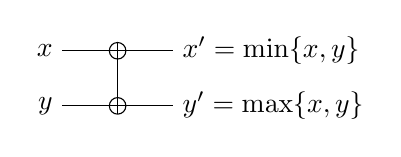
\begin{tikzpicture}[scale=0.7]
    % Draw horizontal lines for x and y
    \draw (-1,1) -- (1,1); % Line for x
    \draw (-1,0) -- (1,0); % Line for y
    
    % Draw vertical line connecting the comparator
    \draw (0,1.15) -- (0,-0.15);
    
    % Draw circles
    \draw (0,1) circle (0.15);
    \draw (0,0) circle (0.15);
    
    % Labels
    \node[left] at (-1,1) {$x$};
    \node[left] at (-1,0) {$y$};
    \node[right] at (1,1) {$x' = \min\{x, y\}$};
    \node[right] at (1,0) {$y' = \max\{x, y\}$};
\end{tikzpicture}
\end{center}

\begin{center}
    \begin{tikzpicture}[scale=0.7]
    % block
    \node[draw, rectangle, minimum width=1.6cm, minimum height=1.2cm] (blk) 
    {\color{red}$\ominus BM[2]$};
    
    % inputs
    \draw
    ($(blk.west)+(-1,0.4)$) node[left] {$x$}
    -- ($(blk.west)+(0,0.4)$);
    \draw
    ($(blk.west)+(-1,-0.4)$) node[left] {$y$}
    -- ($(blk.west)+(0,-0.4)$);
    
    % outputs, shifted up/down by 0.3 units
    \draw
    ($(blk.east)+(0,0.4)$) -- ($(blk.east)+(1,0.4)$)
    node[right] {$x'=\max\{x,y\}$};
    \draw
    ($(blk.east)+(0,-0.4)$) -- ($(blk.east)+(1,-0.4)$)
    node[right] {$y'=\min\{x,y\}$};
\end{tikzpicture}
    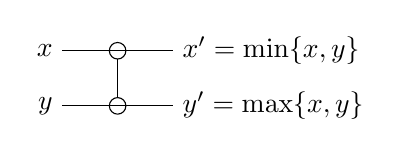
\begin{tikzpicture}[scale=0.7]
    % Draw horizontal lines for x and y
    \draw (-1,1) -- (1,1); % Line for x
    \draw (-1,0) -- (1,0); % Line for y
    
    % Draw vertical line connecting the comparator
    \draw (0,0.85) -- (0,0.15);
    
    % Draw circles
    \draw (0,1) circle (0.15);
    \draw (0,0) circle (0.15);
    
    % Labels
    \node[left] at (-1,1) {$x$};
    \node[left] at (-1,0) {$y$};
    \node[right] at (1,1) {$x' = \min\{x, y\}$};
    \node[right] at (1,0) {$y' = \max\{x, y\}$};
\end{tikzpicture}
\end{center}

Sulla destra una semplificazione in quanto reti con $n = 2$ sono dei comparatori.

Per una rete con $n$ fili, $\oplus BM [n]$, (quindi sequenza bitonica lunga $n$ in ingresso e ordinata in uscita), servono: 
\begin{itemize}
    \item $\log_2 n$ colonne
    \item $n/2$ comparatori per colonna
\end{itemize}

Ogni colonna ha comparatori a distanza pari a metà della colonna precedente (per $n=16$, prima colonna a distanza $8$, seconda a distanza $4$, \dots, fino a distanza 1 in $\log_2 n$ passi). Esempio per rete con $n = 16$:
\begin{center}
    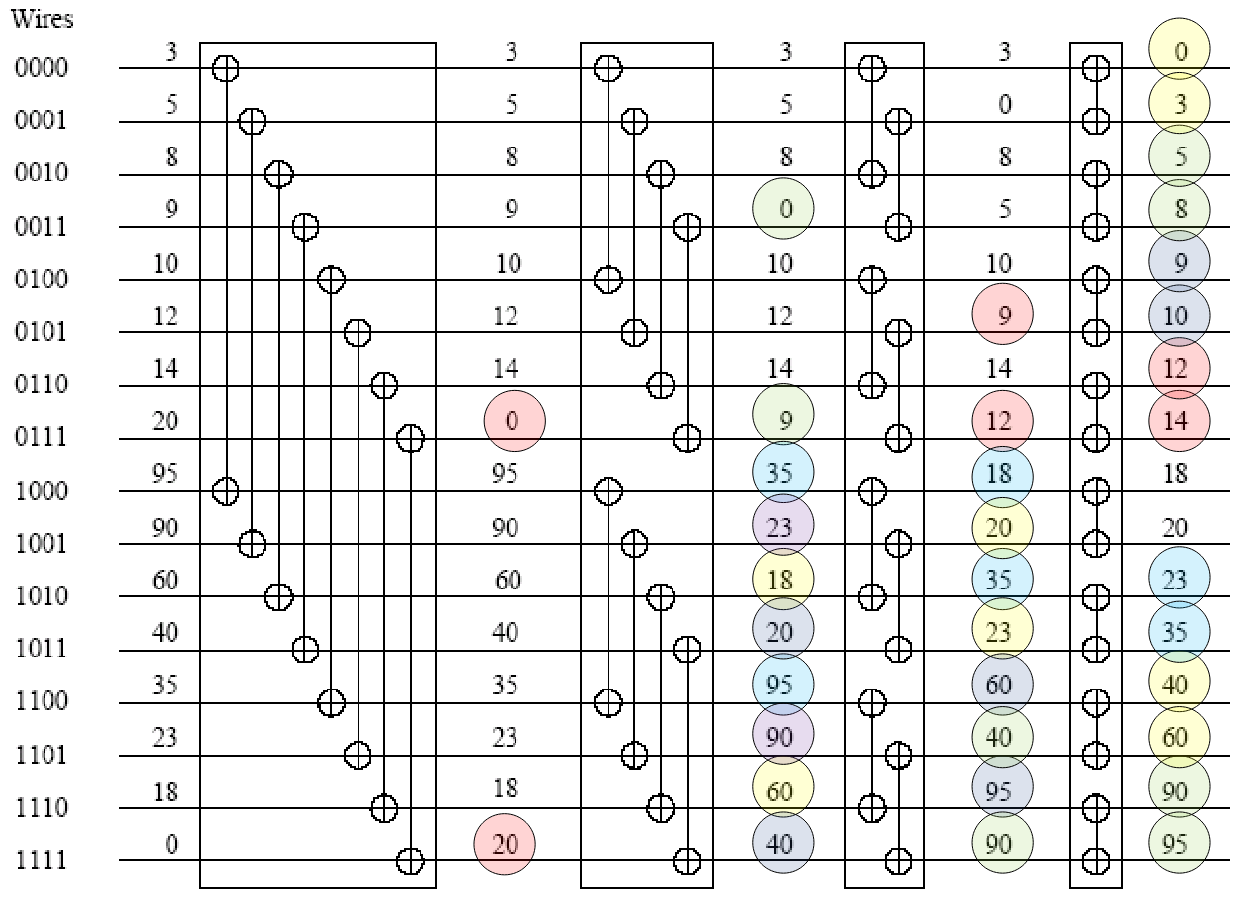
\includegraphics[width=0.79\columnwidth]{img/pattern/n16}
\end{center}

\paragraph{Costruzione di sequenza bitonica:} Con input una sequenza arbitraria, vogliamo ottenere una sequenza bitonica in output. Si può fare alternando i segni dei $BM$.

L'idea è quella di usare una rete con $(\log_2 n) - 1$ colonne: ogni $i$-esima colonna:
\begin{itemize}
    \item prende in input una sequenza bitonica di lunghezza $2^i$, a partire da $i=1$, una sequenza lunga 2 è banalmente bitonica
    
    \item si costruisce una sequenza bitonica lunga $2^{i+1}$ alternando $\oplus BM[2^i]$ con $\ominus BM[2^i]$, da fornire in input alla colonna successiva
\end{itemize}

L'ultima colonna avrà una $\oplus BM [n/2]$ e una $\ominus BM [n/2]$, per creare una sequenza bitonica lunga $n$.

\subsubsection{Ordinamento bitonico}

Si può ordinare una sequenza qualsiasi avendo: 
\begin{itemize}
    \item $(\log n) - 1$ step per costruire una sequenza bitonica a partire dall'input (come visto prima)
    
    \item aggiungere un comparatore $\oplus BM [n]$ alla fine per ordinare la sequenza
\end{itemize}

\paragraph{Complessità:} Per una sequenza lunga $n$, ogni step richiede: 
\begin{align*}
    T(n) & = T(n/2) + \log (n) \\
    & = \log (n) + \log (n/2) + \dots + 1 \\
    & = \sum_{i=0}^{\log n} i \\
    & = \frac{\log n \left((\log n) + 1\right)}{2} \\
    & = \Theta (\log^2 n) 
\end{align*}

%End L10

\end{document}
